%%%%%%%%%%%%%%%%%%%%%%%%%%%%%%%%%%%%

\section{カイ二乗独立性検定}

%%%%%%%%%%%%%%%%%%%%%%%%%%%%%%%%%%%

\subsection{人気のある子供たち}

%%%%%%%%%%%%%%%%%%%%%%%%%%%%%%%%%%%

\begin{frame}[shrink=5]
\frametitle{人気のある子供たち}

\dq{\texttt{popular}データセットでは、4〜6年生が、良い成績・運動能力・人気のどれが最も重要かを尋ねられました。学年と最も重要な要因で分けた二元表を示します。目標が学年によって異なることを示す証拠はありますか？}

\twocol{0.5}{0.5}
{
\begin{center}
\begin{tabular}{rrrr}
  \hline
 & 成績 & 人気 & スポーツ \\
  \hline
$4$年生 &  63 &  31 &  25 \\
$5$年生 &  88 &  55 &  33 \\
$6$年生 &  96 &  55 &  32 \\
   \hline
\end{tabular}
\end{center}
}
{
\begin{center}
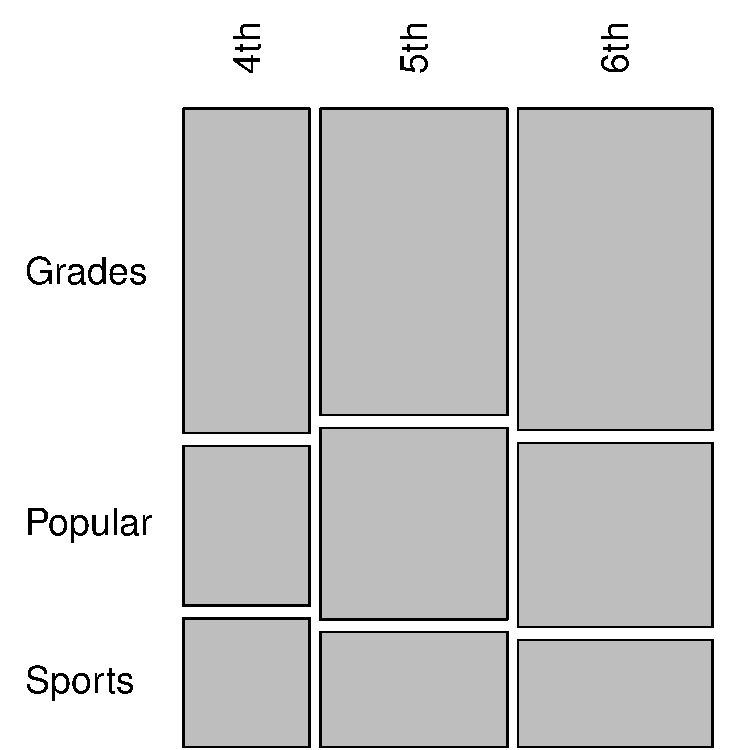
\includegraphics[width=0.75\textwidth]{6-4_chisq_indep/figures/popular/popular_mosaic}
\end{center}
}


\end{frame}

%%%%%%%%%%%%%%%%%%%%%%%%%%%%%%%%%%%

\begin{frame}
\frametitle{カイ二乗独立性検定}

\begin{itemize}
\item 仮説は：
\begin{itemize}
\item[$H_0$:] 学年と目標は独立しています。目標は学年によって異なりません。
\item[$H_A$:] 学年と目標は従属しています。目標は学年によって異なります。
\end{itemize}

\item 検定統計量は次のように計算されます：
\[ \chi^2_{df} = \sum_{i = 1}^{k} \frac{(O - E)^2}{E} \quad \text{ ここで } \quad df = (R - 1) \times (C - 1), \]
ここで$k$はセル数、$R$は行数、$C$は列数です。

\Note{一元表と二元表では$df$の計算が異なります。}

\item p値は$\chi^2_{df}$曲線の、計算された検定統計量より上の面積です。

\end{itemize}


\end{frame}

%%%%%%%%%%%%%%%%%%%%%%%%%%%%%%%%%%%

\subsection{二元表の期待度数}

%%%%%%%%%%%%%%%%%%%%%%%%%%%%%%%%%%%

\begin{frame}
\frametitle{二元表の期待度数}

\formula{二元表の期待度数}
{
\[ \text{期待度数} = \frac{(\text{行合計}) \times (\text{列合計})}{\text{表の合計}} \]
}

{\small
\begin{center}
\begin{tabular}{rrrr|r}
  \hline
 & 成績 & 人気 & スポーツ	& 合計 \\
  \hline
$4$年生 &  \orange{63} &  \green{31} &  25 	&119 \\
$5$年生 &  88 &  55 &  33	& 176 \\
$6$年生&  96 &  55 &  32	& 183 \\
   \hline
合計	& 247	& 141	& 90	& 478 \\
\end{tabular}
\end{center}
}

\[ \orange{$E_{\text{行1,列1}} = \frac{119 \times 247}{478} = 61$} \qquad
 \green{$E_{\text{行1,列2}} = \frac{119 \times 141}{478} = 35$} \]

\end{frame}

%%%%%%%%%%%%%%%%%%%%%%%%%%%%%%%%%%%

\begin{frame}
\frametitle{二元表の期待度数}

\pq{ハイライトされたセルの期待度数は何ですか？}

{\small
\begin{center}
\begin{tabular}{rrrr|r}
  \hline
 & 成績 & 人気 & スポーツ	& 合計 \\
  \hline
$4$年生 &  63 &  31 &  25 	&119 \\
$5$年生 &  88 &  \orange{55} &  33	& 176 \\
$6$年生 &  96 &  55 &  32	& 183 \\
   \hline
合計	& 247	& 141	& 90	& 478 \\
\end{tabular}
\end{center}
}

\twocol{0.2}{0.8}
{
\begin{enumerate}[(a)]
\solnMult{$\frac{176 \times 141}{478}$}
\item $\frac{119 \times 141}{478}$
\item $\frac{176 \times 247}{478}$
\item $\frac{176 \times 478}{478}$
\end{enumerate}
}
{
\soln{
\orange{$\rightarrow$ 52\\
{\small 期待より多くの5年生が \\
人気を目標としている}}
\vspace{0.75cm}
}
}

\end{frame}

%%%%%%%%%%%%%%%%%%%%%%%%%%%%%%%%%%%

\begin{frame}
\frametitle{二元表での検定統計量の計算}

期待度数は観測度数の隣に\ex{青色}で示されています。
\begin{center}
\begin{tabular}{rrrr|r}
  \hline
 & 成績 & 人気 & スポーツ	& 合計 \\
  \hline
$4$年生 	&  63 \ex{61} &  31 \ex{35} &  25 \ex{23}	&119 \\
$5$年生 	&  88 \ex{91} &  55 \ex{52} &  33 \ex{33}	& 176 \\
$6$年生	&  96 \ex{95} &  55 \ex{54} &  32 \ex{34}	& 183 \\
   \hline
合計	& 247	& 141	& 90	& 478 \\
\end{tabular}
\end{center}

\vspace{0.5cm}

\begin{eqnarray*}
\chi^2 &=& \sum \tfrac{(63-61)^2}{61} + \tfrac{(31-35)^2}{35} + \cdots + \tfrac{(32-34)^2}{34} = 1.3121 \\
df &=& (R - 1) \times (C - 1) = (3-1) \times (3-1) = 4
\end{eqnarray*}

\end{frame}

%%%%%%%%%%%%%%%%%%%%%%%%%%%%%%%%%%%

\subsection{結果}

%%%%%%%%%%%%%%%%%%%%%%%%%%%%%%%%%%%

\begin{frame}
\frametitle{p値の計算}

\pq{この仮説検定の正しいp値はどれですか？
\[ \chi^2 = 1.3121 \qquad df = 4 \]
}

\twocol{0.6}{0.4}{
\begin{center}
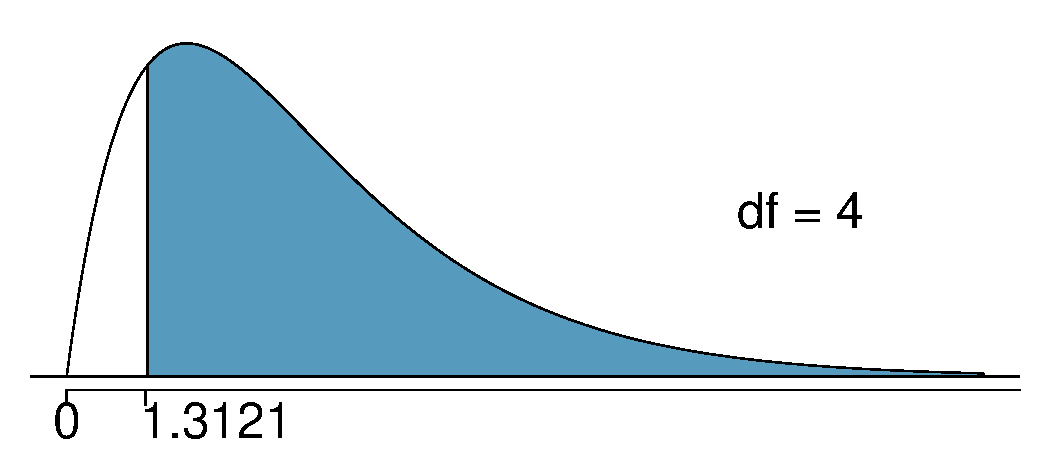
\includegraphics[width=0.67\textwidth]{6-4_chisq_indep/figures/popular/popular}
\end{center}
}
{
{\small
\begin{enumerate}[(a)]
\setlength{\itemsep}{0in}
\solnMult{ 0.3より大きい}
\item 0.3と0.2の間
\item 0.2と0.1の間
\item 0.1と0.05の間
\item 0.001未満
\end{enumerate}
}
}

\end{frame}

%%%%%%%%%%%%%%%%%%%%%%%%%%%%%%%%%%%

\begin{frame}
\frametitle{結論}

\dq{これらのデータは、目標が学年によって異なることを示す証拠を提供しますか？}

\begin{itemize}

\item[$H_0$:] 学年と目標は独立しています。目標は学年によって異なりません。

\item[$H_A$:] 学年と目標は従属しています。目標は学年によって異なります。\\

\end{itemize}

$\:$ \\

\soln{p値が高いため、$H_0$を棄却しません。データは学年と目標が従属しているという説得力のある証拠を提供しません。目標は学年によって異ならないようです。
}

\end{frame}
